\documentclass[11pt,a4paper]{amsart}
\usepackage[utf8]{inputenc}
\usepackage[T1]{fontenc}
\usepackage{lmodern}
\usepackage{amsmath,amssymb,amsthm}
\usepackage{booktabs}
\usepackage{array}
\usepackage{graphicx}
\usepackage[margin=2.3cm]{geometry}
\usepackage{xcolor}
\usepackage[colorlinks=true,linkcolor=blue!50!black,citecolor=blue!50!black,urlcolor=blue!50!black]{hyperref}

\newtheorem{theorem}{Theorem}
\newtheorem{lemma}[theorem]{Lemma}
\newtheorem{proposition}[theorem]{Proposition}
\newtheorem{corollary}[theorem]{Corollary}
\theoremstyle{remark}
\newtheorem*{remark}{Remark}

\setlength{\textfloatsep}{10pt plus 2pt minus 2pt}
\newcommand{\bc}{\mathbf c}
\newcommand{\bX}{\mathbf X}
\newcommand{\E}{\mathbb E}
\newcommand{\Mp}{M^{\mathrm{pr}}}

\title[Permutation, polynomial and saddle-point moments]{A note and restoration on the permutation, polynomial,
and saddle-point moments in \texorpdfstring{\lq\lq Sieve weights and their smoothings\rq\rq}{"Sieve weights and their smoothings"}}
\thanks{Code and data are archived at Zenodo, \href{https://doi.org/10.5281/zenodo.24297078}{doi:10.5281/zenodo.24297078};\\ repository: \href{https://github.com/Ruqing1963/gkm-2021-sieve-weights-audit}{github.com/Ruqing1963/gkm-2021-sieve-weights-audit}.}
\author{Ruqing Chen}
\address{GUT Geoservice Inc., Montreal, Canada}
\email{ruqing@hotmail.com}
\date{November 16, 2026}
\subjclass[2020]{11N36, 11T55, 05A15}
\keywords{sieve weights, M\"obius divisor sums, polynomials over finite fields, random permutations, Poisson moments}

\begin{document}
\begin{abstract}
We check Sections~2.5, 3 and~4 (the permutation and $\mathbb F_q[t]$ analogues) of A.~Granville,
D.~Koukoulopoulos and J.~Maynard, \emph{Sieve weights and their smoothings}.
(i) The divisor sum $M(\bc;m)$ in (3.1) omits the multiplicity $\prod_j\binom{c_j}{b_j}$. As printed,
Proposition~3.1 fails: for $m=1$ the right-hand side is $1-e^{-1}$ for every $k$, whereas $c(1,k)$ is the
Bell number $B_{2k}$. The proof of Theorem~1.4 inherits the unweighted formula through a recurrence on
p.~21. We restore Proposition~3.1 with a short generating-function proof. This gives the Pascal shift
$M(\bc+\mathbf e_i;m)=M(\bc;m)-M(\bc;m-i)$ and a two-line replacement for the end of the proof of
Theorem~1.4. (ii) On p.~20, $\binom{q}{c_1}/(q-1)^{c_1}=\frac1{c_1!}(1+O(c_1/q))$ is claimed for
$c_1\le q$. The true expansion is $\frac1{c_1!}(1-c_1(c_1-3)/(2q)+\cdots)$, and it collapses for
$c_1\gg\sqrt q$. A quadratic Poisson moment repairs the error term, and Theorem~1.4 holds as stated.
(iii) In the heuristic of Section~2.5, three slips lead to the exponent $2^{2k-1}-6k-1$ for the
contribution of $\theta_j\approx\frac12$ to $\mathrm{Poly}_q(n,m,2;k)$. With them corrected the exponent
is $2^{2k-1}-4k-1$. We also prove that $\lim_{q\to\infty}\mathrm{Poly}_q(n,m,2;k)$ is a $2k$-fold mixed
difference of the lattice-point count. Exact values give $15m^2-51m+65$ for $k=2$, and for $k=3$ an
exponent estimated at $20$--$22$, far above $13$. The qualitative conclusions of the paper are unaffected.
\end{abstract}
\maketitle

\section{Introduction}

Let $\mathrm{Poly}_q(n,m;k)=q^{-n}\sum_{\deg N=n}\bigl(\sum_{M\mid N,\ \deg M=m}\mu(M)\bigr)^{2k}$. Theorem~1.4
of \cite{GKM} states that $\mathrm{Poly}_q(n,m;k)=c(m,k)(1+O_k(1/q))$ for $n\ge2mk$. Here $c(m,k)$ is the
number of tuples $(r_S)_{\emptyset\ne S\subset[2k]}$ of non-negative integers with $r_S\in\{0,1\}$ for $|S|$
odd and $\sum_{S\ni i}r_S=m$ for each $i$. We check Section~3 (Proposition~3.1, via permutations), Section~4
(the proof of Theorem~1.4) and the heuristic of Section~2.5.
Page numbers refer to the arXiv version of \cite{GKM} (77 pages).

Throughout, $X_1,\dots,X_m$ are independent with $X_j\sim\mathrm{Poisson}(1/j)$, and
$\bc=(c_1,\dots,c_m)\in\mathbb Z_{\ge0}^m$. All identities were checked symbolically or by exact integer
arithmetic, and all numbers were recomputed, by a program provided as supplementary material. Each repair
is local: the binomial weights restore Proposition~3.1, the restricted range restores the error term of
Theorem~1.4, and the corrected exponent strengthens the conclusion of Section~2.5. Every result of
\cite{GKM} that is used later stands.

\section{Proposition 3.1 and the missing binomial weights}\label{sec:prop31}

Equation (3.1) defines
$\Mp(\bc;m)=\sum_{0\le b_j\le c_j,\ \sum_j jb_j=m}(-1)^{b_1+\dots+b_m}$, and Proposition~3.1 asserts
$c(m,k)=\E[\Mp(\bX;m)^{2k}]$ for every $k$. This is false.
\begin{itemize}
\item For $m=1$, $\Mp((c_1);1)=-\mathbf 1_{c_1\ge1}$, so $\E[\Mp(\bX;1)^{2k}]=\Pr(X_1\ge1)=1-e^{-1}=0.6321\ldots$
for every $k$. But $c(1,k)$ counts the set partitions of $[2k]$, so $c(1,k)=B_{2k}$: $2$, $15$, $203$ for
$k=1,2,3$.
\item For $m=2$, $\Mp=\mathbf 1_{c_1\ge2}-\mathbf 1_{c_2\ge1}\in\{-1,0,1\}$, so for every $k$ the
moment is the probability that exactly one of the two events holds:
\[
\E[\Mp(\bX;2)^{2k}]=e^{-1/2}+2e^{-1}-4e^{-3/2}=0.4498\ldots,
\]
against $c(2,1)=2$ and $c(2,2)=90$.
\item In general $|\Mp(\bc;m)|\le p(m)$, the partition number, so the right-hand side is at most
$p(m)^{2k}$. Table~\ref{tab:mom} gives the values for $m\le4$ and $k\le3$.
\end{itemize}

The source is the count of divisors. A permutation with $c_j$ cycles of length $j$ has
$\prod_j\binom{c_j}{b_j}$ invariant sets made of $b_j$ cycles of length $j$ (p.~18). Likewise, a polynomial
of factorisation type $\bc$ has $\prod_j\binom{c_j}{b_j}$ squarefree divisors of that shape (p.~19). The
divisor sum is therefore
\begin{equation}\label{eq:Mtrue}
M(\bc;\ell)=\sum_{\substack{0\le b_j\le c_j\\ \sum_j jb_j=\ell}}(-1)^{b_1+\dots+b_m}\prod_{j=1}^m\binom{c_j}{b_j}
=[x^\ell]\prod_{j=1}^m(1-x^j)^{c_j}.
\end{equation}
This is not only a misprint in (3.1). The proof of Theorem~1.4 (p.~21) writes
$\Mp(\mathbf e_i+\bc;m)=\Mp(\bc;m)+(-1)^{c_i+1}\Mp(\bc_i;m-i(c_i+1))$, where $\bc_i$ has $i$-th entry $0$.
This identity holds for $\Mp$, but it fails for \eqref{eq:Mtrue}: for example, $M((2);1)=-2$, whereas the
right side gives $-1$. In $305$ of $400$ random tests it fails.

\begin{lemma}\label{lem:gf}
For $\ell_1,\dots,\ell_{2k}\le m$, $\E\bigl[\prod_{i=1}^{2k}M(\bX;\ell_i)\bigr]$ is the coefficient of
$x_1^{\ell_1}\cdots x_{2k}^{\ell_{2k}}$ in
\[
G_k(\mathbf x)=\prod_{|S|\ \mathrm{odd}}(1-x_S)\Big/\prod_{|S|\ \mathrm{even}}(1-x_S),\qquad
x_S=\prod_{i\in S}x_i,
\]
where $S$ runs over the non-empty subsets of $[2k]$. Equivalently, the coefficient of
$\mathbf x^{\mathbf v}$ in $G_k$ is $(-1)^{v_1+\dots+v_{2k}}N(\mathbf v)$. Here $N(\mathbf v)$ counts the tuples $(r_S)$ with $r_S\in\{0,1\}$
for $|S|$ odd, $r_S\ge0$ for $|S|$ even, and $\sum_{S\ni i}r_S=v_i$.
\end{lemma}

\begin{proof}
By \eqref{eq:Mtrue} and $\E[z^{X_j}]=e^{(z-1)/j}$, the generating function is
$\prod_{j\le m}\exp\bigl(\frac1j(\prod_i(1-x_i^j)-1)\bigr)$. Coefficients of degree $\le m$ in each
variable do not change if $j$ runs over all $j\ge1$. Expanding,
$\prod_i(1-x_i^j)-1=\sum_S(-1)^{|S|}x_S^j$, and $\sum_j x_S^j/j=-\log(1-x_S)$. For the sign, note that
$\sum_{|S|\,\mathrm{odd}}r_S\equiv\sum_S|S|r_S-\sum_{|S|\,\mathrm{even}}|S|r_S\equiv\sum_iv_i\pmod 2$.
\end{proof}

Combinatorially, $S$ is the set of indices $i$ whose divisor $G_i$ contains a given cycle (or irreducible
factor), and $r_S$ is the total length assigned to $S$. A cycle of length $j$ contributes
$\mu^{|S|}=(-1)^{|S|}$ and $x_S^j$, and summing over $j$ with the Poisson weights $1/j$ and
exponentiating gives $(1-x_S)^{(-1)^{|S|+1}}$. For even $S$ this is $1/(1-x_S)$, so $r_S\ge0$; for odd
$S$ it is $1-x_S$, so $r_S\in\{0,1\}$. These are exactly the constraints defining $c(m,k)$.

\begin{proposition}[Proposition 3.1, restored]\label{prop:31}
With $M$ as in \eqref{eq:Mtrue}, $c(m,k)=\E[M(\bX;m)^{2k}]$ for all $m,k\ge1$. Moreover, for $1\le i\le m$,
\begin{equation}\label{eq:pascal}
M(\mathbf e_i+\bc;m)=M(\bc;m)-M(\bc;m-i),\qquad M(\bc;0)=1,\quad M(\bc;\ell)=0\ (\ell<0).
\end{equation}
\end{proposition}

\begin{proof}
Take $\ell_i=m$ in Lemma~\ref{lem:gf}. Then $\sum_iv_i=2km$ is even and $N(m,\dots,m)=c(m,k)$. The shift
\eqref{eq:pascal} is \eqref{eq:Mtrue} with $(1-x^i)^{c_i+1}=(1-x^i)^{c_i}-x^i(1-x^i)^{c_i}$.
\end{proof}

The proof avoids permutations entirely. For $m=1$ it reduces to a classical fact: $M((c_1);1)=-c_1$,
and $\E[X_1^{2k}]=B_{2k}$ for $X_1\sim\mathrm{Poisson}(1)$ (Touchard), which is $c(1,k)$. The proof also
confirms Remark~3.1: by exact coefficient extraction,
$3c(m,2)=64m^3-135m^2+182m-66$ for $1\le m\le30$. Table~\ref{tab:mom} compares the two sides; Poisson sums with the weights of \eqref{eq:Mtrue}
reproduce $c(m,k)$ to relative error $<10^{-9}$.

\begin{table}[ht]
\centering\small
\caption{$c(m,k)$ (exact) against $\E[\Mp(\bX;m)^{2k}]$ with $\Mp$ as printed in (3.1).}\label{tab:mom}
\begin{tabular}{r rrr rrr}
\toprule
& \multicolumn{3}{c}{$c(m,k)$} & \multicolumn{3}{c}{$\E[\Mp(\bX;m)^{2k}]$}\\
\cmidrule(lr){2-4}\cmidrule(lr){5-7}
$m$ & $k=1$ & $k=2$ & $k=3$ & $k=1$ & $k=2$ & $k=3$\\
\midrule
1 & 2 & 15 & 203 & 0.6321 & 0.6321 & 0.6321\\
2 & 2 & 90 & 20523 & 0.4498 & 0.4498 & 0.4498\\
3 & 2 & 331 & 1151998 & 0.4538 & 0.6195 & 1.2822\\
4 & 2 & 866 & 40889138 & 0.4569 & 0.7213 & 1.7790\\
\bottomrule
\end{tabular}
\end{table}

\emph{The end of the proof of Theorem~1.4 (p.~21).} It must be shown that
$T_i:=\E[X_iM(\bX;m)^{2k}]\ll_kc(m,k)$. Since $\E[X_if(\bX)]=\frac1i\E[f(\bX+\mathbf e_i)]$ for Poisson
variables, \eqref{eq:pascal} and $(a-b)^{2k}\le2^{2k-1}(a^{2k}+b^{2k})$ give
\[
T_i=\frac1i\E\bigl[(M(\bX;m)-M(\bX;m-i))^{2k}\bigr]\le\frac{2^{2k-1}}{i}\bigl(c(m,k)+c(m-i,k)\bigr)\le\frac{4^k}{i}\,c(m,k).
\]
Here $c(0,k)=1$, and the monotonicity of $c(\cdot,k)$ is Lemma~1.5. This replaces the argument with
$\bc_i$ on p.~21.

\section{The binomial ratio on p.~20}\label{sec:ratio}

For $j=1$ (so $N_1=q$), p.~20 states
$\binom{N_1}{c_1}(q-1)^{-c_1}=\frac1{c_1!}(1+O(c_1/q))$ for $c_1\le q$. In fact
\[
\frac{c_1!\binom{q}{c_1}}{(q-1)^{c_1}}=\prod_{i<c_1}\Bigl(1-\frac iq\Bigr)\Bigl(1-\frac1q\Bigr)^{-c_1}
=1-\frac{c_1(c_1-3)}{2q}+O\Bigl(\frac{c_1^4}{q^2}\Bigr)\qquad(c_1\le\sqrt q).
\]
The step $(1+O(c_1/N_1))^{c_1}=1+O(c_1/q)$ is valid only for bounded $c_1$. For $c_1\gg\sqrt q$ the ratio is
of size $e^{-c_1^2/(2q)}$, and at $c_1=q$ it equals $e^{1-q}\sqrt{2\pi q}\,(1+o(1))$. For $q=10^6$ and
$c_1=3\sqrt q$, $|{\rm ratio}-1|\,q/c_1=330$. The inset of Figure~\ref{fig:main}(b) shows the collapse
on the scale $c_1/\sqrt q$.

\begin{proposition}\label{prop:ratio}
In Section~4 of \cite{GKM}, restrict the main-term range to the vectors $\bc$ with $c_1\le\sqrt q$
and $\sum_{j\ge2}c_j\,(j/q^j)^{1/2}\le1$. Replace $(c_1+1)/q$ by $(c_1^2+1)/q$ in $E_1$ and $E_2$, and the
condition $c_1>q$ by $c_1>\sqrt q$ in $E_2$ and $E_3$. Then $E_1+E_2+E_3\ll_kc(m,k)/q$, and Theorem~1.4
holds as stated.
\end{proposition}

\begin{proof}
On the new range the ratio is $\frac1{c_1!}(1+O(c_1^2/q))$. Off it, $c_1^2/q>1$, so $E_2$ is bounded as on
p.~20. On p.~21, $E_3$ uses only $\binom{q}{c_1}\le(1-1/q)^{-q}(q-1)^{c_1}/c_1!$, which holds for all
$c_1$. It remains to bound $\E[X_1^2M^{2k}]=\E[X_1(X_1-1)M^{2k}]+T_1$. Applying the Poisson identity twice,
and then \eqref{eq:pascal} twice,
\[
\E[X_1(X_1-1)M(\bX;m)^{2k}]=\E\bigl[(M(\bX;m)-2M(\bX;m-1)+M(\bX;m-2))^{2k}\bigr]\le16^k\,c(m,k).
\]
The last step uses convexity with weights $\frac14,\frac12,\frac14$ and the monotonicity of $c(\cdot,k)$.
\end{proof}

\begin{figure}[t]
\centering
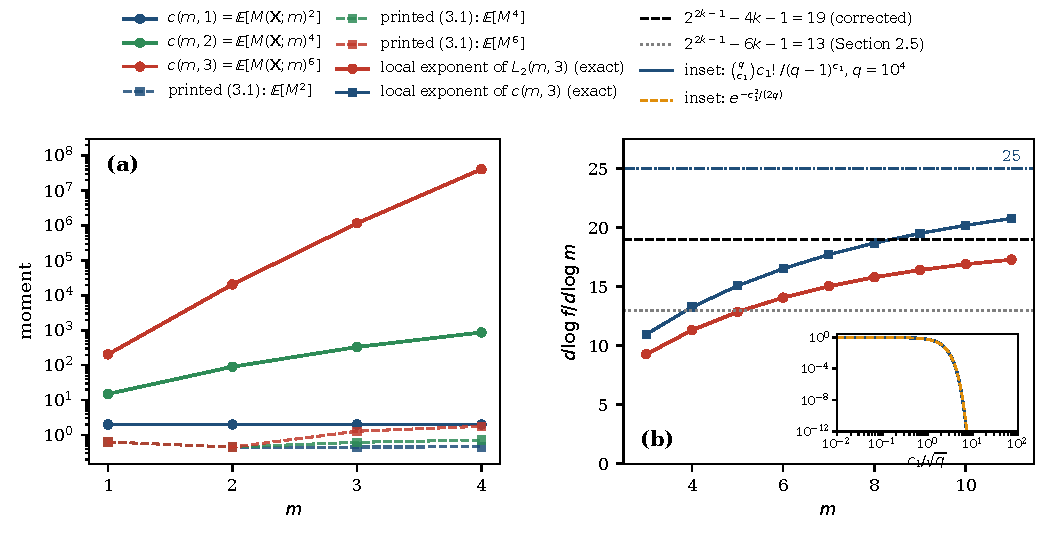
\includegraphics[width=0.76\textwidth]{figures/fig_gkm_2021_audit.pdf}
\caption{(a) $c(m,k)$ with the weights \eqref{eq:Mtrue} (solid) and moments of the printed (3.1)
(dashed). (b) Local exponents of the exact $L_2(m,3)$ and $c(m,3)$. Inset: the ratio of
Section~\ref{sec:ratio} for $q=10^4$.}\label{fig:main}
\end{figure}

\section{Section 2.5: the exponent at \texorpdfstring{$\theta_j\approx\frac12$}{theta = 1/2}}\label{sec:25}

In the integral for $\mathrm{Poly}_q(n,m,2;k)$ (pp.~14--15, $r=1-1/m$, $\mathcal Z_q(w)=(1-w)^{-1}$) the
$j$-th factor is $e(-m\theta_j)r^{-m}(1+re(\theta_j))$, and the region $|\theta_j-\frac12|\le\frac1m$ is
estimated as $m^{2^{2k-1}-6k-1}$. With $\theta_j=\frac12+w_j/m$, $|w_j|\le1$, there are three slips.
\begin{enumerate}
\item The Taylor step expands $1+e(\theta_j)$, and omits $2\pi i$. The correct factor is
$1+re(\theta_j)=(1-2\pi iw_j)/m+O(m^{-2})$, which does not vanish at $w_j=0$.
\item The factors $\mathcal Z_q(r^{|I|}e(\theta_I))$, $I\in\mathcal S^+(2k)$, are treated as
$m^{2^{2k-1}-1}(1+O(1/m))$ on the whole region. They equal $m/(|I|-2\pi iw_I)+O(1)$, so they vary by
bounded factors and couple the variables through $w_I=\sum_{j\in I}w_j$. Likewise
$e(-m\theta_j)=e(-m/2)e(-w_j)$ is not constant.
\item Because of (2), the terms linear in each $w_j$ do not cancel \lq\lq by symmetry\rq\rq, and the
quadratic terms do not give the main contribution. For $k=2$, the rescaled integral
\[
J_2=\int_{[-1,1]^4}\prod_{|I|\,\mathrm{even}}\frac1{|I|-2\pi iw_I}\prod_{j=1}^4e(-w_j)(1-2\pi iw_j)\,dw
\]
is $0.0482$; with the paper's factor $-2\pi iw_j$ in place of $1-2\pi iw_j$ it is $0.0434$, not $0$.
\end{enumerate}
So the region contributes $\asymp m^{(2^{2k-1}-1)-2k-2k}J_k=m^{2^{2k-1}-4k-1}J_k$, a factor $m^{2k}$
more than stated. But the cut-off $|w_j|\le1$ is arbitrary (the $w$-integral is not absolutely convergent
on $\mathbb R^{2k}$), so the order of $\mathrm{Poly}_q(n,m,2;k)$ needs the following identity.

\begin{proposition}\label{prop:L2}
Let $L_2(m,k):=\E\bigl[(M(\bX;m)+M(\bX;m-1))^{2k}\bigr]$. Then
\[
L_2(m,k)=\sum_{\boldsymbol\varepsilon\in\{0,1\}^{2k}}(-1)^{|\boldsymbol\varepsilon|}\,N(m-\varepsilon_1,\dots,m-\varepsilon_{2k}),
\]
with $N$ as in Lemma~\ref{lem:gf}. Section~4 of \cite{GKM}, corrected as above and applied to
$M(\bc;m)+M(\bc;m-1)$, gives $\mathrm{Poly}_q(n,m,2;k)=L_2(m,k)+O_k(c(m,k)/q)$ for $n\ge2mk$.
\end{proposition}

\begin{proof}
Take the coefficient of $x_1^m\cdots x_{2k}^m$ in $\prod_i(1+x_i)\,G_k(\mathbf x)$ (Lemma~\ref{lem:gf}).
\end{proof}

Thus $L_2(m,k)=\lim_{q\to\infty}\mathrm{Poly}_q(n,m,2;k)$ is the $2k$-fold mixed backward difference of $N$
at $(m,\dots,m)$: multiplying by $1+x_i$ adds the coefficient at $v_i-1$, and the sign $(-1)^{\sum v}$
turns this sum into $N(\mathbf v)-N(\mathbf v-\mathbf e_i)$, as $\sum_i(m-\varepsilon_i)\equiv|\boldsymbol\varepsilon|\pmod2$. Geometrically, $N(\mathbf v)$ counts the
lattice points of a polytope with right-hand side $\mathbf v$. Up to a constant, its smooth part is the
volume polynomial $V$, of degree $2^{2k-1}-2k-1$, and the $2k$ differences pick out
$\partial_1\cdots\partial_{2k}V$, of degree $2^{2k-1}-4k-1$, unless it vanishes. Lower-dimensional strata
can dominate. Exact coefficient extraction in $G_k$ (modulo two $61$-bit primes for $k=3$, checked with a
second pair) gives, for $k=2,$
\[
L_2(m,2)=15m^2-51m+65\qquad(3\le m\le30),
\]
of order $m^2$, whereas both region exponents are negative ($-1$, $-5$), as the paper anticipates for small
$k$. For $k=3$, the local exponent of $L_2(m,3)$ rises from $9.3$ at $m=3$ to $17.3$ at $m=11$
(Figure~\ref{fig:main}(b)). Fitting $D+a/m+b/m^2(+c/m^3)$ to the local exponents gives $D\in[20.4,22.1]$.
On $c(m,3)$, whose exponent is $25$, the same fits give $[24.8,27.9]$. The data are consistent with
$2^{5}-12-1=19$ and well above $13$. The conclusion of Section~2.5 is unaffected and in fact
strengthened. Table~\ref{tab:sum} summarises all points.

\begin{table}[!ht]
\centering\footnotesize
\caption{Status of the points checked in \cite{GKM} (arXiv page numbers).}\label{tab:sum}
\begin{tabular}{lll}
\toprule
Location & Issue & Status after repair\\
\midrule
(3.1), p.~17 & weights $\prod_j\binom{c_j}{b_j}$ omitted & Prop.~3.1 true only with \eqref{eq:Mtrue} (Prop.~\ref{prop:31})\\
Prop.~3.1, p.~18 & divisor count uses (3.1) & new proof via Lemma~\ref{lem:gf}\\
Thm.~1.4, p.~21 & recurrence for unweighted $M$ & Pascal shift \eqref{eq:pascal}; $T_i\le4^kc(m,k)/i$\\
Thm.~1.4, p.~20 & $1+O(c_1/q)$ for $c_1\le q$ & $O(c_1^2/q)$ for $c_1\le\sqrt q$; Thm.~1.4 holds (Prop.~\ref{prop:ratio})\\
Rem.~3.1, p.~17 & formula for $c(m,2)$ & verified for $1\le m\le30$\\
Sec.~2.5, pp.~14--15 & exponent $2^{2k-1}-6k-1$ & $2^{2k-1}-4k-1$ for the region; exact $L_2$ (Prop.~\ref{prop:L2})\\
\bottomrule
\end{tabular}
\end{table}
\begin{thebibliography}{9}
\bibitem{GKM} A.~Granville, D.~Koukoulopoulos and J.~Maynard, \emph{Sieve weights and their smoothings},
Ann.\ Sci.\ \'Ec.\ Norm.\ Sup\'er.\ (4) \textbf{54} (2021), no.~5, 1089--1177; arXiv:1606.06781.
\end{thebibliography}
\end{document}
